\setchapterpreamble[u]{\margintoc}
\chapter{Second Lecture}
\labch{lec2}

\newcolumntype{C}[1]{
	 >{\vbox to 3ex\bgroup\vfill\centering}
	 p{#1}<{\egroup}
}

\newcommand{\tabularRow}[2]{
	\multicolumn{4}{l}{#1}\\[+1em]
	\includegraphics[width=0.4\textwidth]{#2 (before)}&
	% https://www.pngrepo.com/svg/41763/rotated-right-arrow-with-broken-line 
	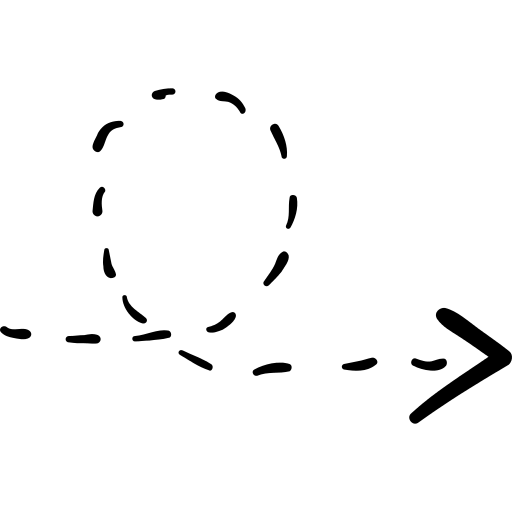
\includegraphics[width=0.1\textwidth]{lec2/Rotated Right Arrow (pngrepo.com)} &
	\includegraphics[width=0.4\textwidth]{#2 (after)}\\
}

\section[Intro. to Mathematical Models]{Introduction to Mathematical Models}
\labsec{sec2.1}
We will be studying single output linear continuous systems. If a system has more than one input
the superposition principle will be applied.\\[-2em]


\subsection[Super Position Principle]{Super Position Principle\linkC{https://en.wikipedia.org/wiki/Superposition_principle}}
 The superposition property, states that, for all linear systems, the net response caused by two
 or more stimuli is the sum of the responses that would have been caused by each stimulus individually.\\[+1em]
\hspace*{\fill}\fbox{
		    \parbox{3.8cm}{
		    $\ F(x_1 + x_2) = F(x_1) + F(x_2)$
	    	}
}\\[+1em]
\note{It can be used to prove linearity}\\[-3em]


\subsection[Simple Systems Equations]{Simple Systems Equations\linkT{Reference: Feedback control system analysis and synthesis}}
The purpose of this section is to present methods of writing the differential equations for a variety of electrical and mechanical systems.
This is the first step that must be mastered by the would-be control systems engineer.\\[-1em]


Series Resistor-Inductor-Capacitor Circuit\\[-1mm]
\begin{marginfigure}[-1em]
		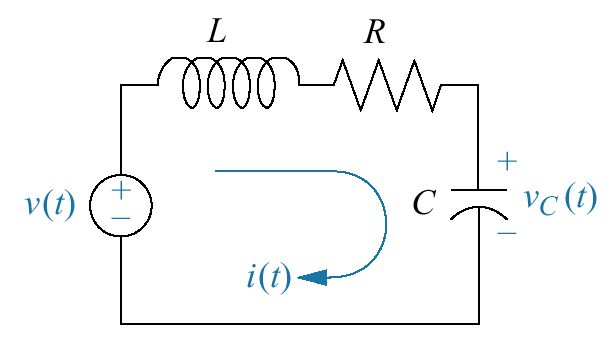
\includegraphics{lec2/Series Resistor-Inductor-Capacitor Circuit}
		\caption{Simple electrical system.}
\end{marginfigure}

\begin{tabular}{C{1mm} C{1mm} C{2cm} l l}
			&$v_L$& $=$ & $(LD)\ i$ &\\
			&$v_R$& $=$ & $R\ i$	&\\
			&$v_C$& $=$ & $(\dfrac{1}{CD})\ i$&\\
			&&&&
\end{tabular}

\vspace{-4em}
\hspace*{\fill}\fbox{
			    \parbox{3.2cm}{
			    $v = (LD + R + \dfrac{1}{CD})\ i$
		    		}
}\\[+2mm]
\note{$R:\ resistor,\ L:\ inductor,\ C:\ capacitor$}\\[-1em]


Simple Mechanical Translation System\\[-1mm]
\begin{marginfigure}[-1em]
		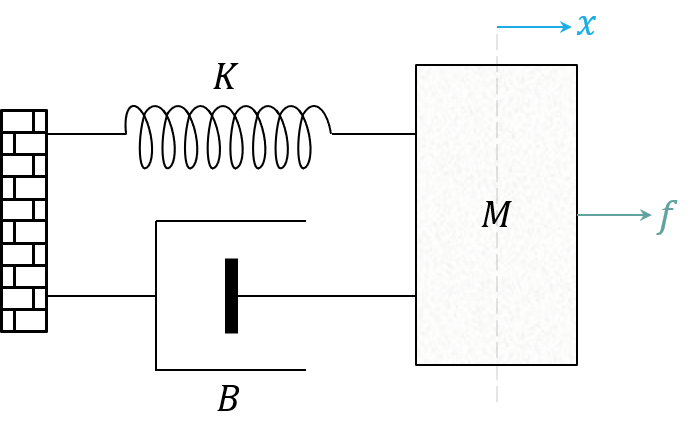
\includegraphics{lec2/Simple Mechanical Translation System}
		\caption{Mechanical translation system.}
\end{marginfigure}

\begin{tabular}{C{1mm} C{1mm} C{2cm} l l}
			&$f_M$& $=$ & $(MD^2)\ x$ &\\
			&$f_B$& $=$ & $(BD)\ x$	&\\
			&$f_K$& $=$ & $K\ x$&\\
\end{tabular}

\vspace{-1em}
\hspace*{\fill}\fbox{
			    \parbox{3.5cm}{
			    $f = (MD^2+BD+K)\ x$
		    		}
}\\[+2mm]
\note{$M:\ mass,\ B:\ damping\ or\ viscous\ friction,\ K:elastance\ or\ stiffness$}\\

\pagebreak

Simple Mechanical Rotational System\\[-1mm]
\begin{marginfigure}[-1em]
		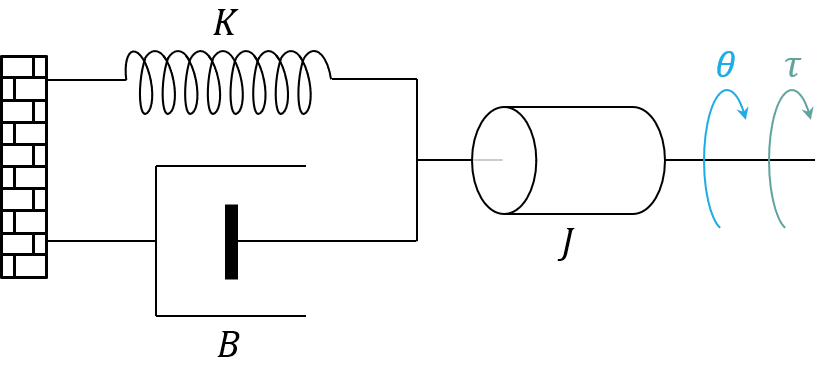
\includegraphics{lec2/Simple Mechanical Rotational System}
		\caption{Mechanical rotational system.}
\end{marginfigure}

\begin{tabular}{C{1mm} C{1mm} C{2cm} l l}
			&$\tau_J$& $=$ & $(JD^2)\ \theta$ &\\
			&$\tau_B$& $=$ & $(BD)\ \theta$	&\\
			&$\tau_K$& $=$ & $K\ \theta$&\\
\end{tabular}

\vspace{-1em}
\hspace*{\fill}\fbox{
			    \parbox{3.3cm}{
			    $\tau = (JD^2+BD+K)\ \theta$
		    		}
}\\[+2mm]
\note{$J:\ moment\ of\ inertia$}\\[-1.5em]


Single-stage Rotating Amplifier\\[-1mm]
\begin{marginfigure}[-1em]
		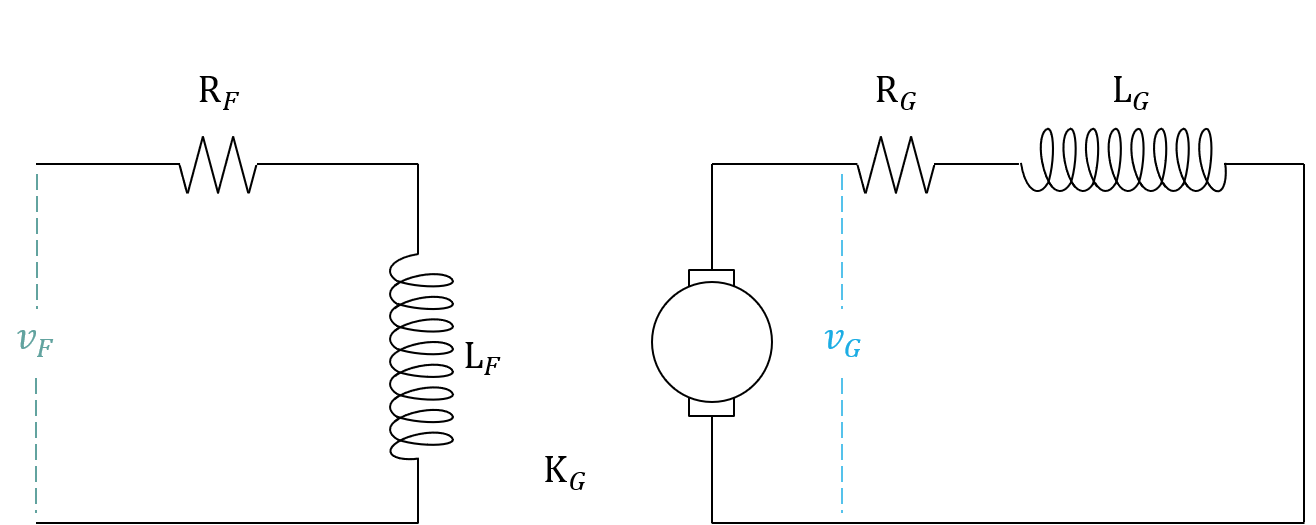
\includegraphics{lec2/Field controlled generator}
		\caption{Field controlled generator.}
\end{marginfigure}

\begin{tabular}{C{1mm} C{1mm} C{2cm} l l}
			&$v_F$& $=$ & $(DL_F+R_F)\ i_F$ &\\
			&$v_G$& $=$ & $K_G\ i_F$&\\
\end{tabular}

\vspace{-1em}
\hspace*{\fill}\fbox{
			    \parbox{3.1cm}{
			    $v_F = (\dfrac{DL_F+R_F}{K_G})\ v_G$
		    		}
}\\[+2mm]
\note{$F:\ field,\ G:\ generator$}\\[-1.5em]

D-C Servomotor\\[-1mm]
\todo{\tiny{Keep in mind the mechanical rotational system equation.}}

Armature Controlled Motor\\[-1mm]
\begin{marginfigure}[-1em]
		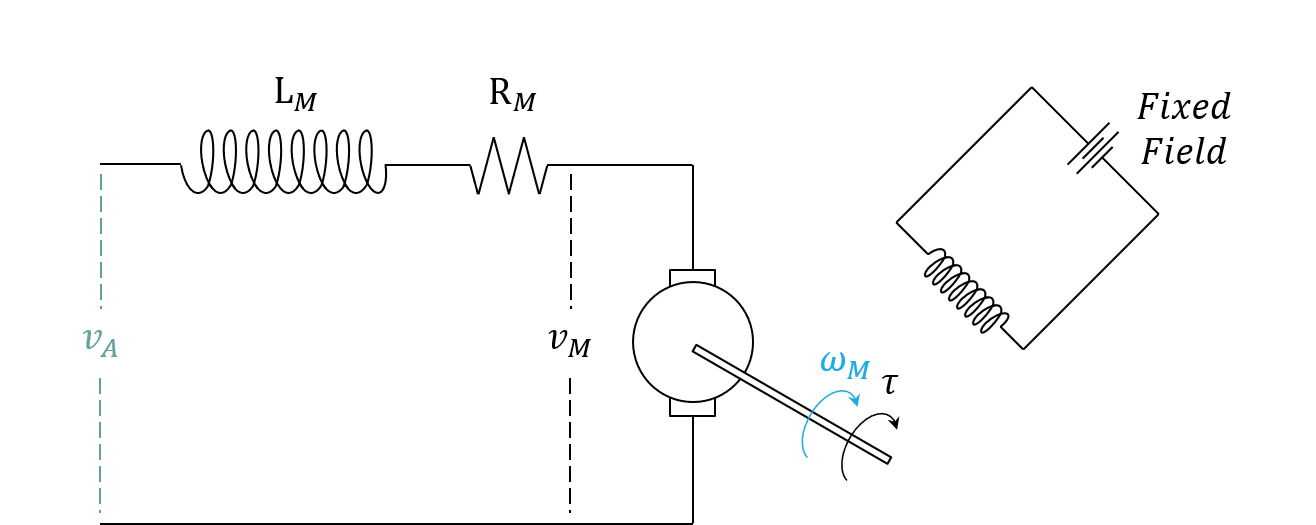
\includegraphics{lec2/Armature controlled motor}
		\caption{Armature controlled motor.}
\end{marginfigure}

\begin{tabular}{C{1mm} C{1mm} C{2cm} l l}
			&$v_M$ & $=$ & $(K_b\ D)\ \theta_M$ &\\
			&$\tau$& $=$ & $K_T\ i_M$ &\\
			&$i_M$ & $=$ & $(\dfrac{JD^2+BD}{K_T})\ \theta_M$ &\\
			&$v_A$ & $=$ & $v_M + (L_M D+R_M)\ i_M$ &\\
\end{tabular}

\vspace{-1em}
\hspace*{\fill}\fbox{
			    \parbox{9.1cm}{
			    $v_A = [\dfrac{(L_M J)\ D^3 + (L_M B+R_M J)\ D^2 + (R_M B + K_b K_T)\ D}{K_T}]\ \theta_M$
		    		}
}\\[+2mm]
\note{$M:\ motor,\ A:\ armature$}\\[-1.5em]

Field Controlled Motor\\[-1mm]
\begin{marginfigure}[-1em]
		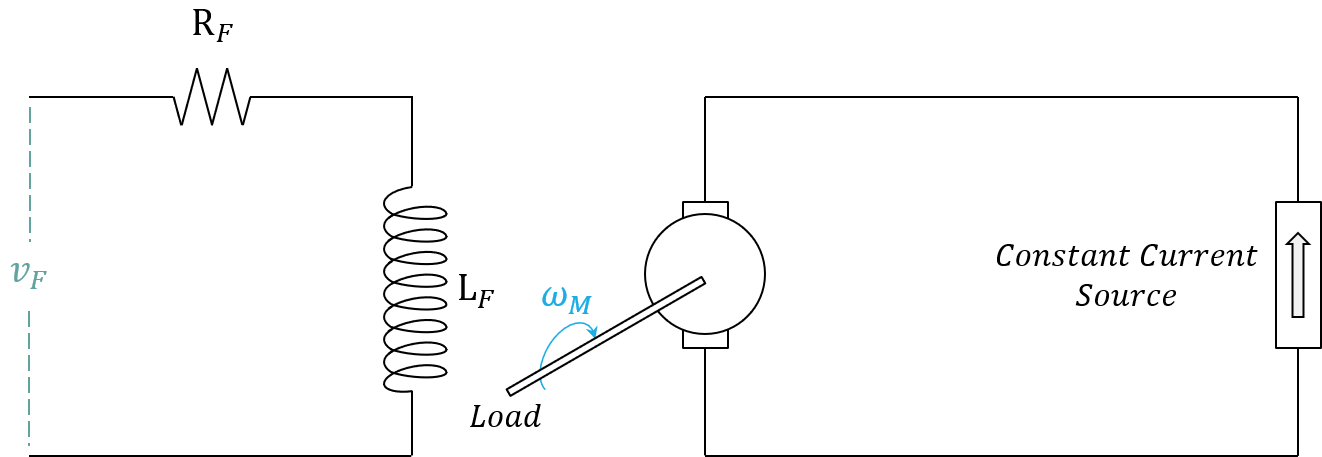
\includegraphics{lec2/Field controlled motor}
		\caption{Field controlled motor.}
\end{marginfigure}

\begin{tabular}{C{1mm} C{1mm} C{2cm} l l}
			&$\tau$& $=$ & $K_F\ i_F$ &\\
			&$i_F $& $=$ & $(\dfrac{JD^2+BD}{K_F})\ \theta_M$ &\\
			&$v_F $& $=$ & $(DL_F+R_F)\ i_F$&\\
\end{tabular}

\vspace{-1em}
\hspace*{\fill}\fbox{
			    \parbox{5.2cm}{
			    $v_F = [\dfrac{(JD^2+BD)(DL_F+R_F)}{K_F}]\ \theta_M$
		    		}
}\\

\section[Block Diagram Reduction $_{p\ 2}$]{Reduction Techniques (Moving Points)}
\labsec{sec2.2}

\raggedleft
\begin{tabular}{m{4cm} m{1cm} m{4cm}}
	\tabularRow{Summing point behind a block:}{lec2/Summing behind}
	\tabularRow{Summing point ahead a block:}{lec2/Summing ahead}
	\tabularRow{Take-off point behind a block:}{lec2/Pickoff behind}
	\tabularRow{Take-off point ahead a block:}{lec2/Pickoff ahead}
\end{tabular}

\vspace{1em}
\begin{description}
\item[Homework] Convert Motor-generator control schematic diagram to block diagram and simpify it.
\end{description}

\begin{figure*}[h!]
	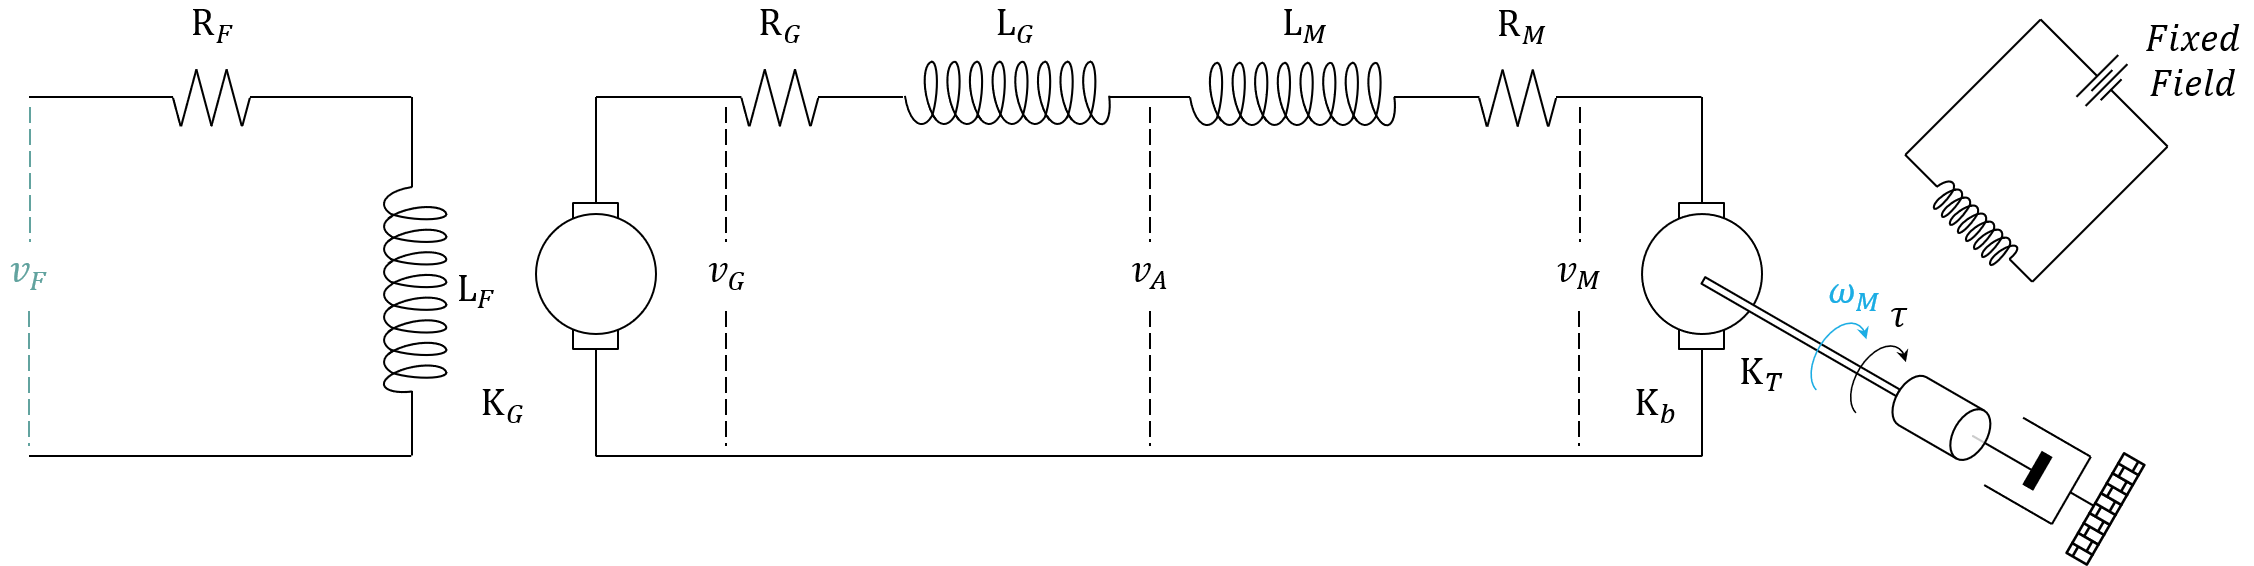
\includegraphics{lec2/Homework}
	\caption{Motor-generator control.}
\end{figure*}

\begin{marginfigure}\scriptsize
		\begin{description}
			\item[Hint] The last step should be:
		\end{description}
		\raggedleft
		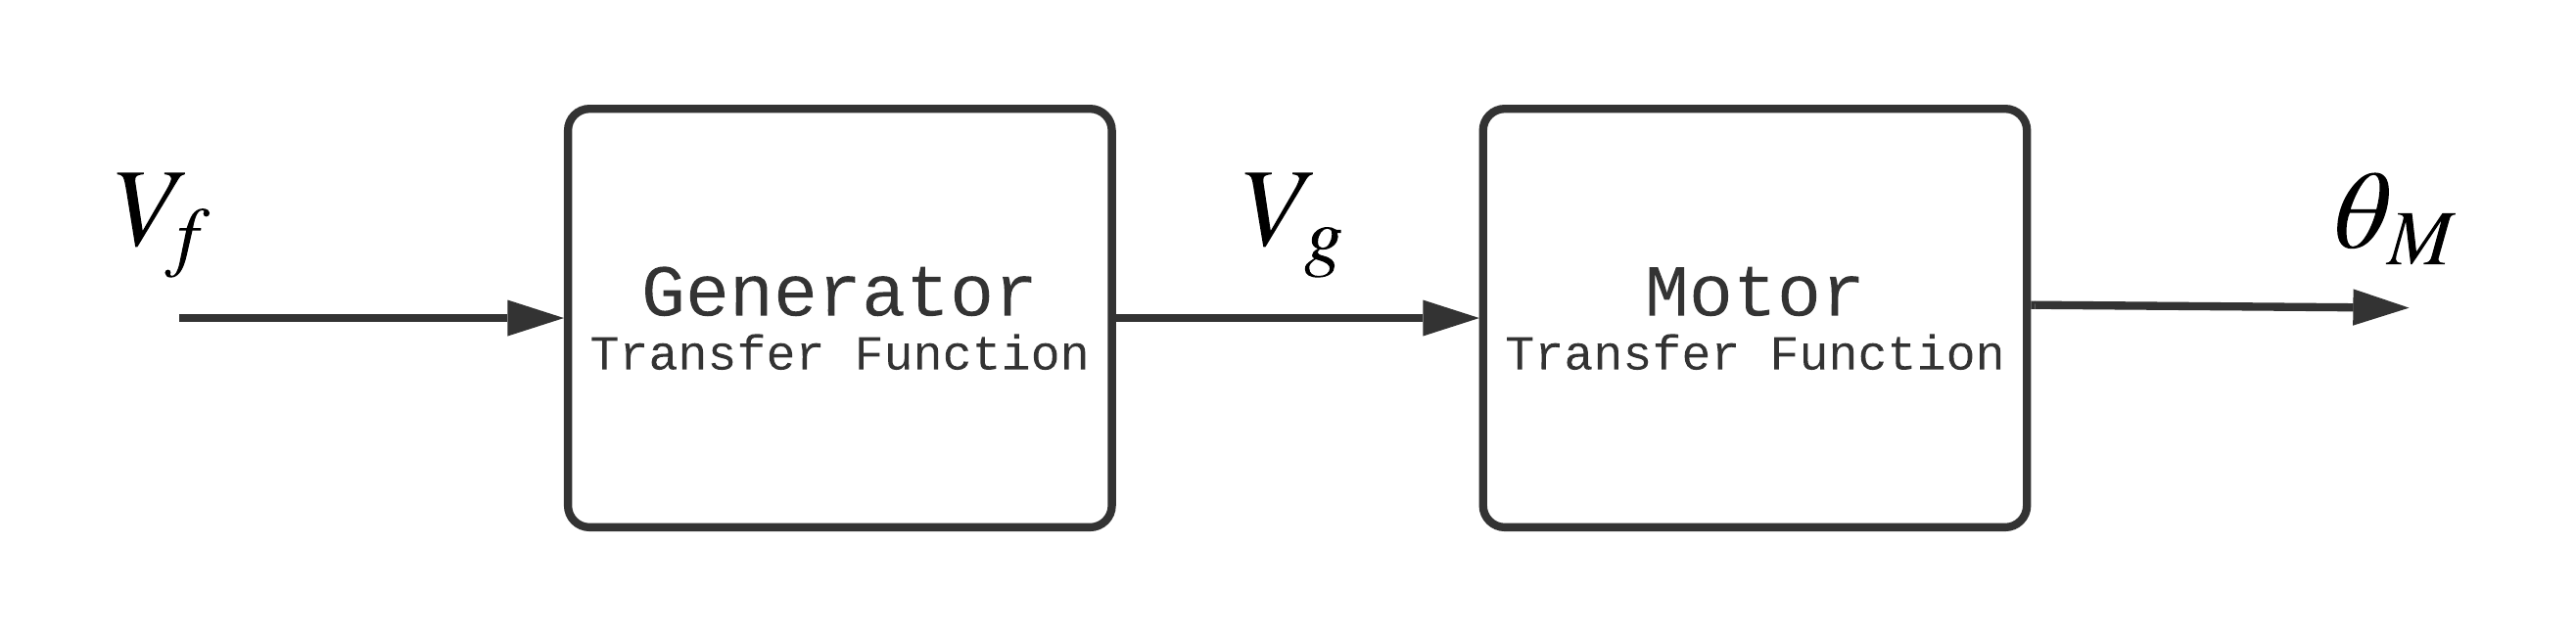
\includegraphics{lec2/Hint}
\end{marginfigure}

\justify % https://www.overleaf.com/learn/latex/Text_alignment#Fully_justified_text